\subsection{Simulations}
A Monte Carlo simulation has been constructed to study the various contributions to the measured resolution.  An example output is shown in Fig.~\ref{sims}. To produce the figures discussed in this section, the simulation included a uniform spherical scattering distribution and a finite beam spot.  Specifically, the beam spot has been simulated as a symmetric Gaussian distribution with 90\% of the beam falling within a radius of $\rho=1.0$\,mm ($\sigma = 0.608$\,mm). This beam spot size was selected to be conservatively large and yet physically reasonable.
\subsubsection{Contributions}
One of the purposes of studying the detector via a simulation was to deconvolve the various contributions to the detector resolution. The results of the simulation study indicate that the observed detector resolution is dominated by the intrinsic detector resolution.  As discussed in Section~\ref{cal_def}, the contribution of the transverse extent of particle trajectories is less than 170\,$\mu$m at the edges of the detector. Near the center of the detector, the contribution approaches zero. These effects are neglected in all of the simulations.

To isolate the contribution of the beam spot size, simulations were run neglecting the effects of beam scattering and detector resolution. Fig.~\ref{sims} shows the simulated position spectra from detector 2.  Comparing Fig.~\ref{sims} with Fig.~\ref{hxc}, one sees that the beam spot size has a minimal contribution to the measured detector resolution. This is not surprising given the distance between the target and the detectors (682.9\,mm) and reasonably-assumed size of the beam spot (1--2\,mm). In order to reproduce the observed resolution in Fig.~\ref{hxc} from the contribution of the beam spot alone, physically unrealistic beam spot sizes are required. For example, a beam spot greater than the size of the target foil is required.
\begin{figure}%
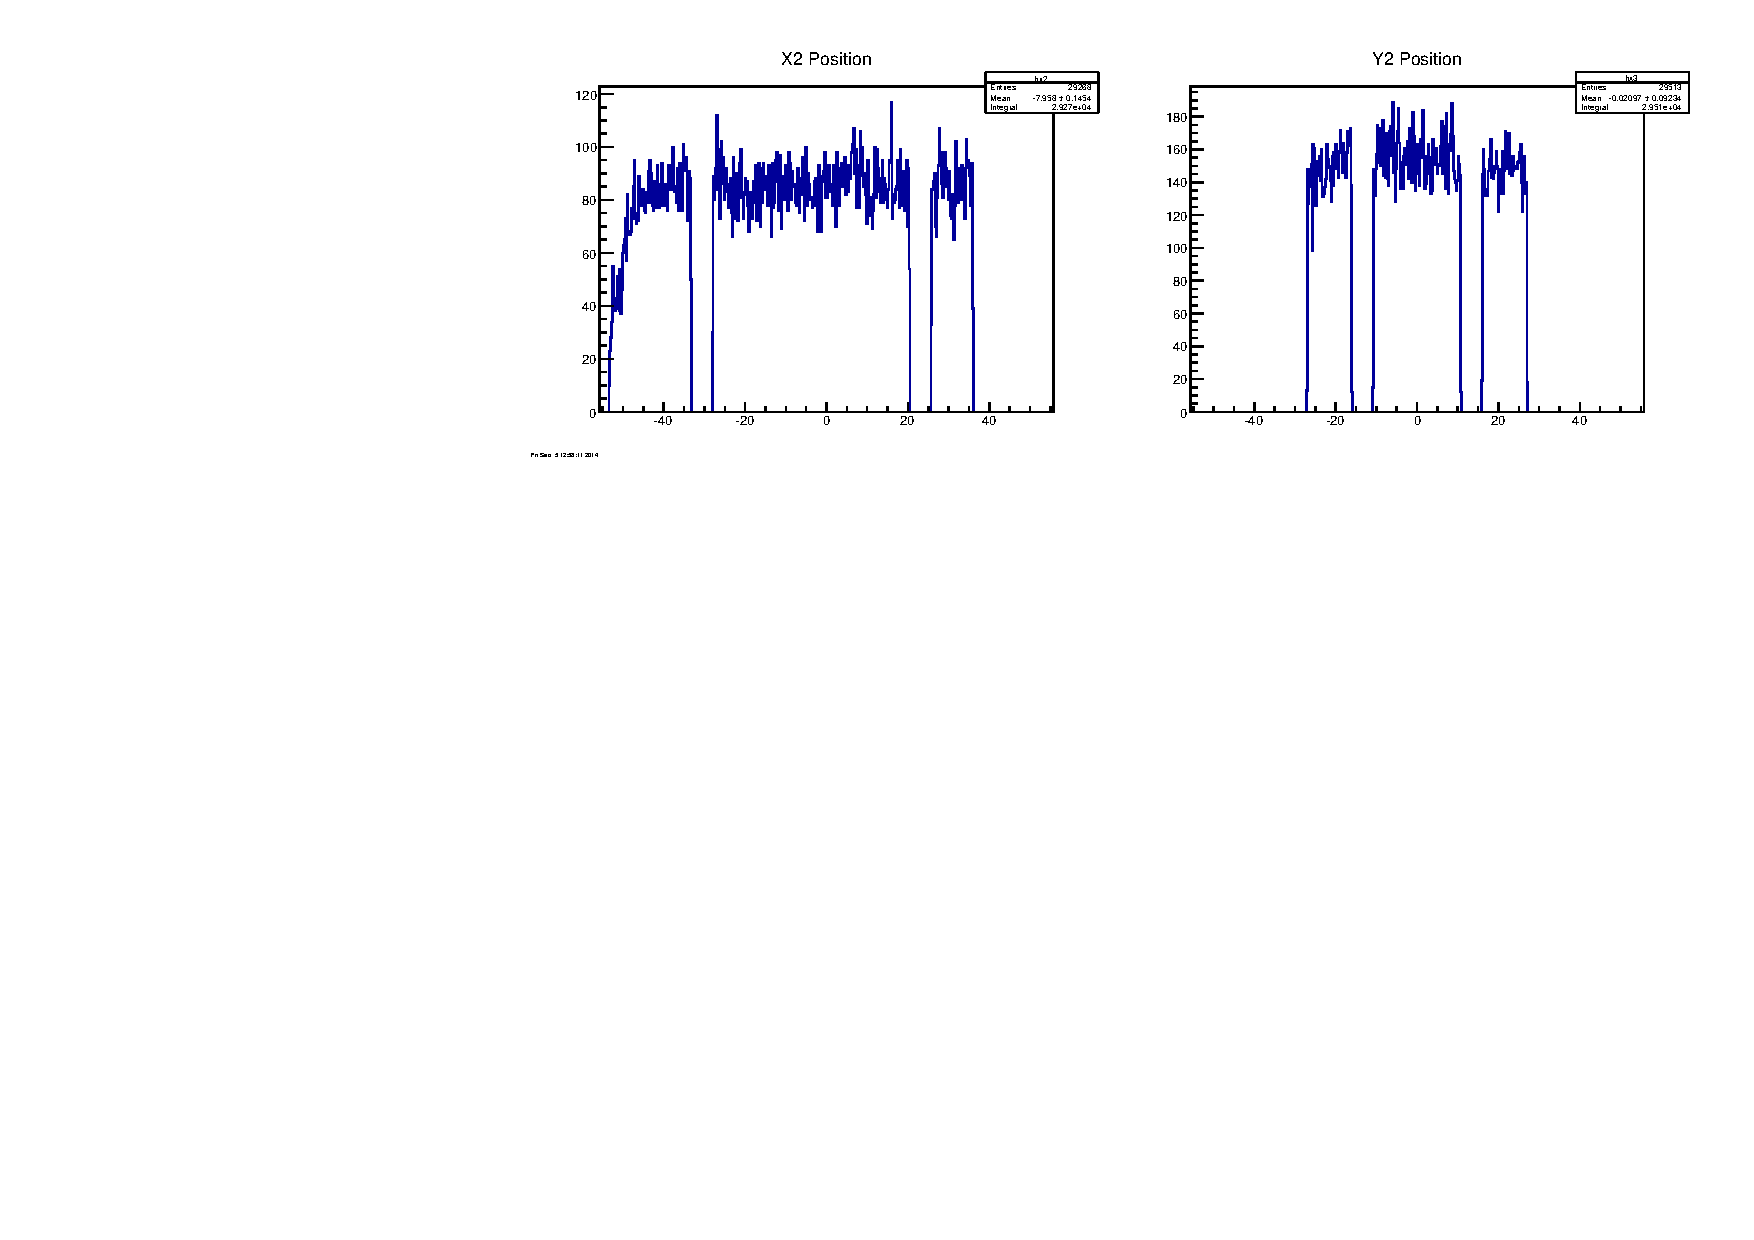
\includegraphics[width=\columnwidth]{sims}%
\caption{Simulated positions spectra of detector 2.}%
\label{sims}%
\end{figure}

\subsubsection{Fitting the Data}
The determination of the detector resolution is accomplished by fitting the data with the simulation. The position of the beam spot is accounted for by geometrically aligning the features of the simulation with those the data. Once the simulation is aligned to the data, the measurement resolution of the simulation is varied to match the shape of the data. Fig.~\ref{sim_comp} show the result of fitting the data with the simulation in order to determine the position resolution of the detector. Because the simulation adequately reproduces the data without including edge scattering, implementation of that effect is neglected. In this example, the data was best fit with a simulated intrinsic detector resolution of 1.3\,mm (3.06\,mm~FWHM).  This fit is consistent with the dubious edge-fitting method presenting in the previous section. For an example such as this, where the wires are not resolved, the quality of the fit of the simulation could be improved on the order of 8\% by including a realistic angular distribution.
\begin{figure}%
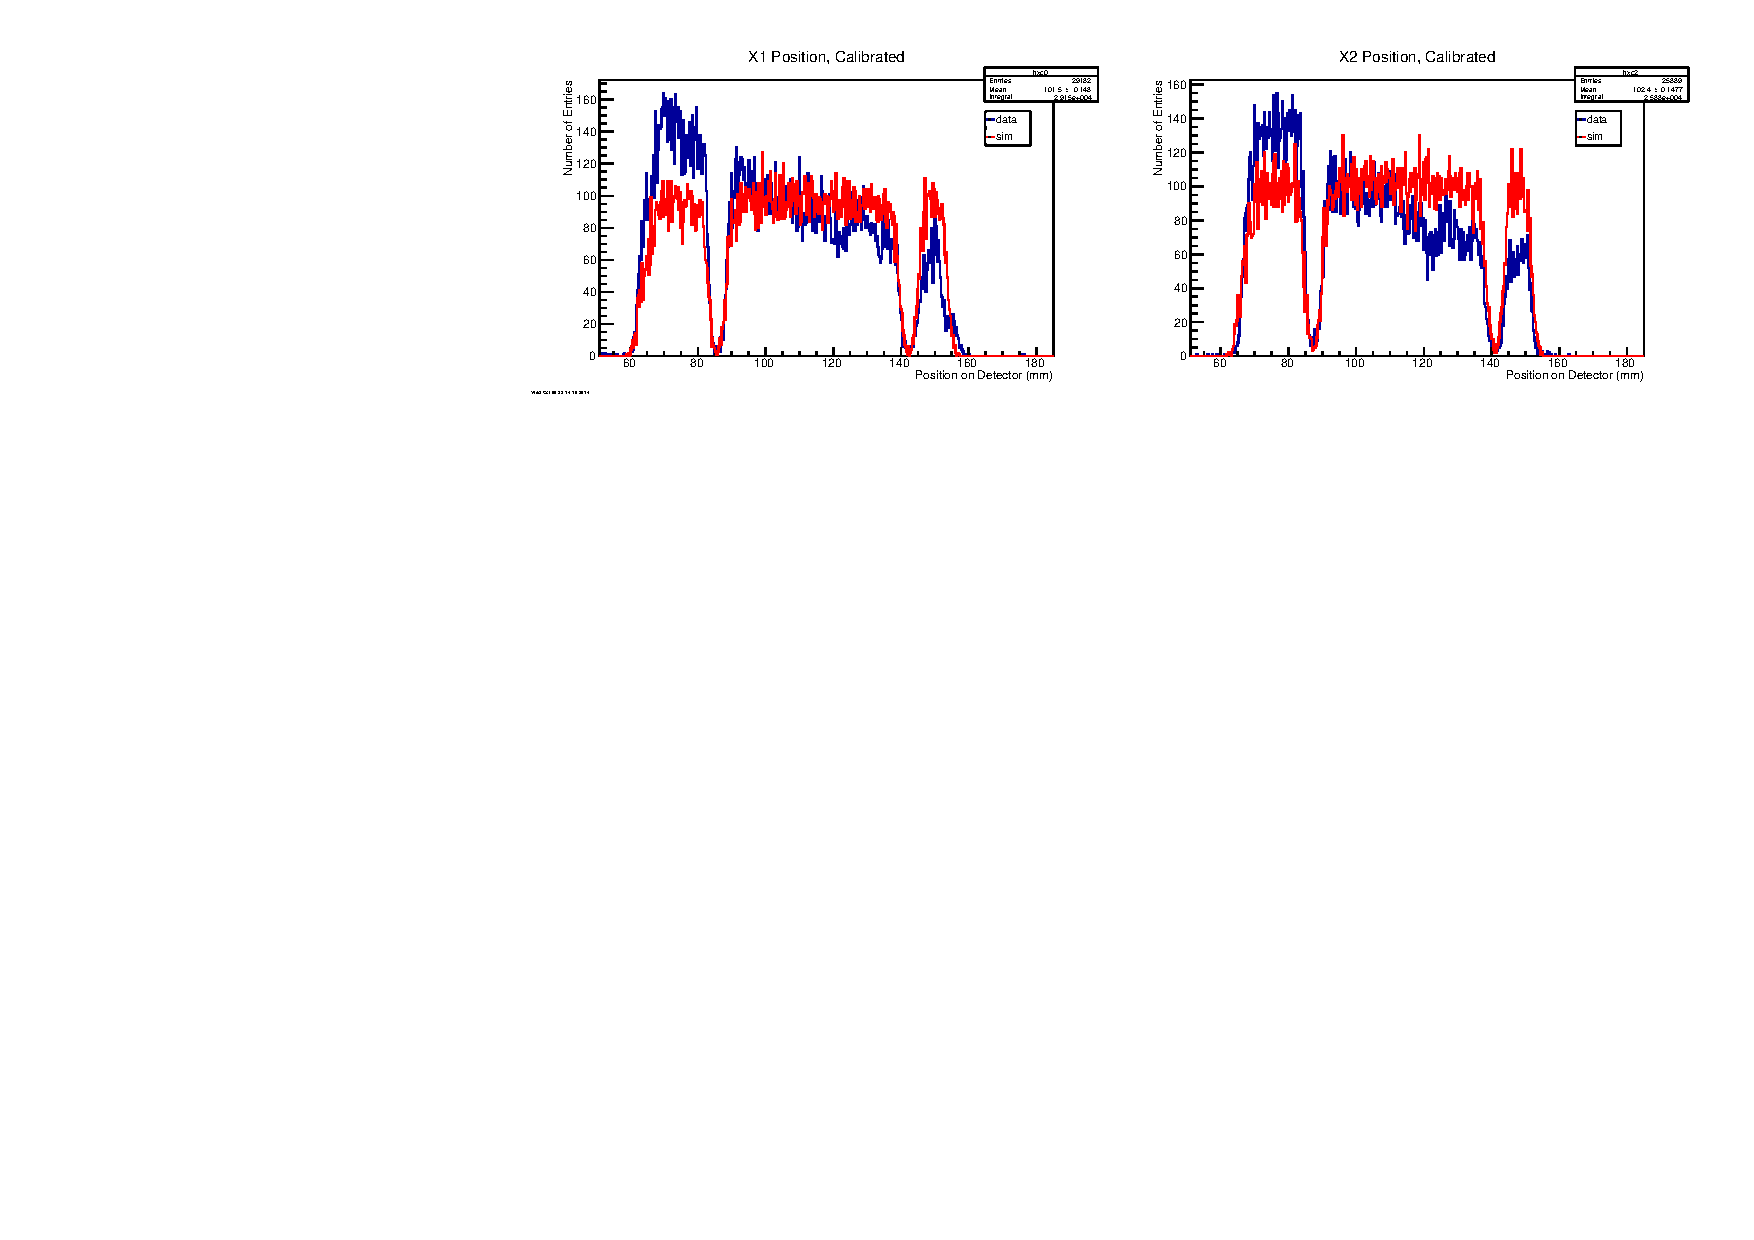
\includegraphics[width=\columnwidth]{run_480_compX}%
\caption{Simulated and measured $x$-position spectra of for each detector. The data (blue) have been fit with a simulated spectra using the following assumptions: a 1.43\,mm~FWHM beam spot centered at the origin and a detector resolution of 1.3\,mm (3.06\,mm~FWHM).}%
\label{sim_comp}%
\end{figure}


